\documentclass[border=10pt]{standalone}

\usepackage{pgfplots}
\pgfplotsset{compat=1.18}
\usepgfplotslibrary{fillbetween}

\begin{document}

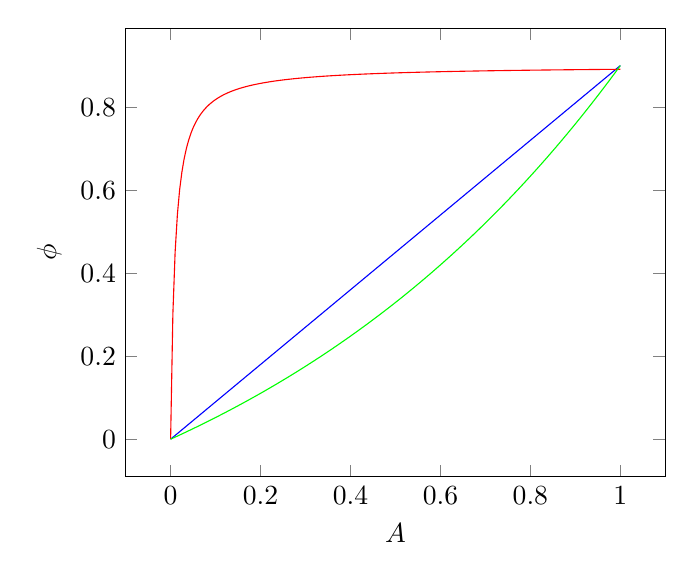
\begin{tikzpicture}
    \begin{axis}
    [xlabel={$A$}, 
    ylabel={$\phi$}, 
    samples  = 200]
        \addplot[ domain = 0:1, color = blue] {.9*x};
        \addplot[ domain = 0:1, color = red] {0.9/(0.01/x+1};
        \addplot[ domain = 0:1, color = green] {0.9/(1-3)*(1-3^x)};
        % \addplot[ domain = 0:1, color = green] {1+ln(exp(x−2)+1)};
        % \addplot[name path = floor, draw = none] coordinates {(-1,0) (1,0)};
        % \addplot[color=gray] fill between[of = parab and floor];
    \end{axis}
\end{tikzpicture}

\end{document}